\documentclass[11pt,twoside]{article}
\usepackage[bf,small]{caption}
\usepackage[letterpaper,hmargin=1in,vmargin=1in]{geometry}
\usepackage{paralist} % comapctitem, compactdesc, compactenum
\usepackage{titlesec}
\usepackage{titletoc}
\usepackage{times}
\usepackage{hyperref}
\usepackage{algorithmic}
%\usepackage{glossaries}
%\usepackage[xindy]{glossaries}
%\usepackage[toc]{glossaries}
\usepackage{graphicx}
\graphicspath{{./graphics/}}
\usepackage{xspace}
\usepackage{verbatim}
\hyphenation{Sub-Bytes Shift-Rows Mix-Col-umns Add-Round-Key}

\setlength{\parskip}{10pt}
\setlength{\parindent}{0pt}

%commonly used terms that require special formatting
\newcommand \bulk {\textit{bulk\_extractor}\xspace}
\newcommand \hdb {\textit{hashdb}\xspace}
\newcommand \hdbm {\textit{hashdb\_manager}\xspace}
\newcommand \hdbc {\textit{hashdb\_checker}\xspace}
\newcommand \hid {\textit{hashid}\xspace}

\begin{document}

\title{User Guide for the \hdb Tools}
\author{Bruce Allen \footnote{\href{mailto:bdallen@nps.edu}{bdallen@nps.edu}}}
\maketitle

\section{Introduction}
The \hdb tools are used for finding blacklist data in raw media
by using chunk hashes.
Chunk hashes are hashes computed from chunks of data
and are typically 4KiB in size.
The \hdb tools provide two fundamental services:
\begin{compactitem}
	\item Creating and maintaining hash databases
	\item Scanning media for matching hash values
\end{compactitem}

Figure~\ref{fig:create_hashdb} illustrates creating a new hash database.
Figure~\ref{fig:scan_hashdb} illustrates scanning a hash database
for hash features.
\begin{figure}[h]
	\center
	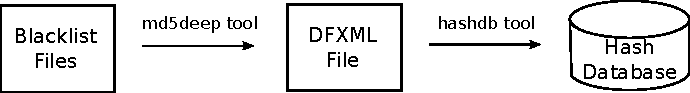
\includegraphics[scale=1.0]{drawings/create_hashdb.pdf}
	\caption{Creating a new hash database}
	\label{fig:create_hashdb}
\end{figure}
\begin{figure}[h]
	\center
	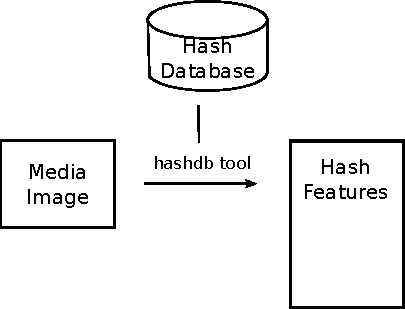
\includegraphics[scale=1.0]{drawings/scan_hashdb.pdf}
	\caption{Scanning a disk image for hash features}
	\label{fig:scan_hashdb}
\end{figure}

\section{Terminology}

\subsection{Chunk Hash}
A chunk hash is a hash of a chunk of data,
typically 4KiB in size.
We copy chunk hashes, along with information of where the chunk values
are sourced from, into a hash database.
We then search through media images for matching chunk hash values
using the \bulk \hid scanner.

To increase the probability of finding chunk hashes in sector-based
disk images, we generate chunk hashes at each sector boundary.
Figure~\ref{fig:sector_boundaries} illustrates chunk hashes
from 4KiB chunks of data aligned on 512 byte sector boundaries.
\begin{figure}[h]
	\center
	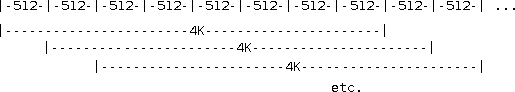
\includegraphics[scale=1.0]{drawings/sector_boundaries.pdf}
	\caption{4KiB chunks of data aligned on 512 byte sector boundaries}
	\label{fig:sector_boundaries}
\end{figure}

\subsection{Hash Source}
Hashes stored in hash databases may be sourced from many files
and from many repositories.
Each source is identified by:
\begin{compactitem}
	\item Repository name
	\item Filename
	\item Offset in the file
\end{compactitem}

A particular hash value may be sourced from multiple places,
be it in other repositories, other files,
or even multiple places in a single file.

\subsection{Hash Database Attribution}
Hash database attribution is provided through history logs
as commands are issued to add, merge, or remove information.
The attribution is stored in XML format under the \hdb directory
in file \texttt{history.xml}.

\subsection{Bloom Filters}
Hash databases can be be large.
Bloom filters may be used to improve performance during hash lookups.
Bloom filters are used to quickly indicate when a hash value
is not in a hash database,
which is expected to be the case most of the time.
If a Bloom filter indicates that a hash value might be in the hash database,
then a database lookup is required to be certain.

\section{\hdb Toolset}
The hashdb toolset consists of the following:
\begin{compactitem}
\item The \hdbm tool, providing \hdb management capabilities:
\begin{compactitem}
\item Import hashes into a \hdb from DFXML input.
\item Copy, append, merge \hdb databases.
\item Track \hdb attribution.
\item Provide remote lookup services over TCP.
\end{compactitem}
\item The \hdb library (\texttt{hashdb.hpp}, \texttt{libhashdb}),
providing an API to programatically interface with the \hdb for hash lookups.
Interfaces support the following \hdb lookup services:
\begin{compactitem}
\item Searching for matching hash values.
\item Identifying where hash values come from.
\item Obtaining information about the \hdb.
\end{compactitem}

The \bulk \hid scanner demonstrates use of this scanner
by interfacing with the \hdb library
to provide hash lookup services, see Section~\ref{hid-scanner}.
Note that the \bulk \hid scanner is distributed with \bulk, not with \hid.
\end{compactitem}

\subsection{\hdbm Usage}
The \hdbm tool provides commands for creating and managing hash databases
and for providing a hash database query service over a socket:

\begin{compactitem}
\item \texttt{copy}: Import a DFXML file into a \hdb
or copy hashes from one \hdb into another.
\item \texttt{remove}: Remove hashes in a DFXML file
or a \hdb from another \hdb.
\item \texttt{merge}: Merge the contents of two {\hdb} databases
into a third \hdb.
\item \texttt{rebuild\_bloom}: Rebuild the bloom filter of a hashdb
to a different size in order to improve lookup performance.
\item \texttt{export}: Export the hashes in a \hdb out to a DFXML file.
\item \texttt{info}: Print out information about a \hdb.
\item \texttt{server}: Provide a query lookup service for a \hdb.
\end{compactitem}

The complete \hdbm usage is listed in Appendix~\ref{hdbm-usage}.

This command line example demonstrates use of the \texttt{md5deep} tool
to create DFXML file \texttt{my\_dfxml\_file}
containing chunk hashes from files under directory \texttt{my\_dir}
and then importing those hash values into a new hash database
named \texttt{my\_hashdb}:

\begin{small}
\begin{verbatim}
hashdb_checker --query_source -q use_path \
-p my_hashdb identified_blocks.txt
\end{verbatim}
\end{small}

\subsection{\hdbc Usage}
In \hdb v1.0.0, query lookup services are provided by a separate \hdbc tool.
This tool provides the following services:

\begin{compactitem}	
\item \texttt{query\_hash}: Query a \hdb for hash values.
\item \texttt{query\_source}: Query source information
from a list of hash values.
\end{compactitem}

The complete \hdbc usage is listed in Appendix~\ref{hdbc-usage}.

The command line example below illustrates the process of
looking up hash sources
from a hash database called \texttt{my\_hashdb}
from a feature file called \texttt{identified\_blocks.txt}
that was created  while using the \bulk \hid scanner:

\begin{small}
\begin{verbatim}
md5deep -p 4096 -d -r my_dir > my_dfxml_file
hashdb_manager --copy my_dfxml_file my_hashdb
\end{verbatim}
\end{small}

\subsection{\hdb Library Usage}
The \hdb library provides an API allowing \hdb query services including:
\begin{compactitem}	
\item \texttt{query\_hashes\_md5}: Check the \hdb for matching MD5 hashes.
\item \texttt{query\_sources\_md5}: Look up source information
for the given MD5 hashes.
\item \texttt{query\_hashdb\_info}: Obtain information about the \hdb.
\end{compactitem}	

The complete \hdb library file \texttt{hashdb.hpp}
is listed in Appendix~\ref{hdb-lib}.

\section{\bulk \hid Scanner\label{hid-scanner}}
The \bulk \hid scanner is not distributed with \hdb; it is part of \bulk.

The \bulk \hid scanner finds matching chunk hash values in media image files.
Matching hash values are stored in the \texttt{identified\_blocks.txt}
feature file.

The \bulk \hid scanner accepts the following inputs
on the \bulk command line:

\begin{compactitem}	
\item \texttt{query\_type}: Selects how the query will be sourced.
Available options:
\begin{compactitem}	
\item \texttt{use\_path}: Specifies that the \hdb used will be at a file path.
\item \texttt{use\_socket}: Specifies that the \hdb used will be
available as a server service available at a socket.
\end{compactitem}	
\item \texttt{path}: Specifies the file path to the \hdb.
\item \texttt{socket}: Specifies the socket endpoint to the \hdb server service.
\item \texttt{chunk\_size}: Specifies a chunk size, in bytes,
to use for generating chunk hashes, default 4096.
\item \texttt{sector\_size}: Specifies a sector size.
Hashes are generated on each sector size boundary.
\end{compactitem}

\subsection{Example using Path}

The command line example below illustrates the process of scanning
disk image file \texttt{my\_imagefile}
for chunk hash values that match values present
in the \texttt{my\_hashdb} hash database and placing
matches in feature file \texttt{identified\_blocks.txt}
under output directory \texttt{outpath}:

\begin{small}
\begin{verbatim}
bulk_extractor -S query_type=use_path \
-S path=my_hashdb -o outpath my_imagefile
\end{verbatim}
\end{small}

It is useful to see where hash values are sourced from.
This command line example illustrates the process of
using the \hdbc tool to obtain
hash source information from the hash values present in \bulk Feature file
\texttt{identified\_blocks.txt} referencing the \hdb
at path \texttt{my\_hashdb}:

\begin{small}
\begin{verbatim}
hashdb_checker --query_source -q use_path -p my_hashdb identified_blocks.txt
\end{verbatim}
\end{small}

\subsection{Example using Socket}
It is beneficial to use a socket when the hash database is large
because it takes time for the hash database to open.
It is additionally beneficial to use the socket across systems
in order to keep as much of the hash database cached in memory as possible,
for faster performance.

This example has several parts.
First, it opens a socket server service
enabling queries against a hash database.
Then it performs query functions against the database that is available
over the socket service.

The command line example below illustrates the process of opening
hash database \texttt{my\_hashdb} as a separate
query service process running in a separate terminal window
available at default socket \texttt{tcp://*:14500}
using the \hdbm tool:

\begin{small}
\begin{verbatim}
hashdb_manager --server my_hashdb
\end{verbatim}
\end{small}

The command line example below illustrates the process of scanning
disk image file \texttt{my\_imagefile}
for chunk hash values that match values present
in the \texttt{my\_hashdb} hash database
made available as a socket service in the example above.
Hash values that match the hash database are placed
in feature file \texttt{identified\_blocks.txt}
under output directory \texttt{outpath}:

\begin{small}
\begin{verbatim}
bulk_extractor -S query_type=use_socket -o outpath my_imagefile
\end{verbatim}
\end{small}

It is useful to see where hash values are sourced from.
This command line example illustrates the process of
using the \hdbc tool to obtain
hash source information from the hash values present in \bulk Feature file
\texttt{identified\_blocks.txt} referencing the socket service opened above:

\begin{small}
\begin{verbatim}
hashdb_checker --query_source -q use_socket identified_blocks.txt
\end{verbatim}
\end{small}


% no, later:
%When the \bulk \hid scanner finds matching hashes,
%it only records the matching hash value.
%To determine the source of hash values,
%perform a post\-processing source lookup.
%In \hdb v1.0.0, this lookup is performed using a separate \hdbc tool.

% *************************** Appendix ****************************
\appendix
\section{Usage}
\subsection{\hdbm Usage\label{hdbm-usage}}
The complete \hdbm usage,
obtained by typing \texttt{hashdb\_manager -H}, follows:
\begin{small}
\begin{verbatim}
hashdb_manager Version 1.0.0
Usage: hashdb_manager -h | -H | -V | <command>
    -h, --help    print this message
    -H            print detailed help including usage notes and examples
    --Version     print version number

hashdb_manager supports the following <command> options:

--copy [<hashdb tuning parameter>]+ [-r <repository name>] <input> <hashdb>
    Copies the hashes in the <input> into the <hashdb> hash database.

    Options:
    <hashdb tuning parameter>
        When a new <hashdb> hash database is being created,
        <hashdb tuning parameter> options may be provided to configure the
        hash database.  Please see <hashdb tuning parameter> options and
        <bloom filter tuning parameter> options for settings and default
        values.

    -r, --repository=<repository name>
        When importing hashes from a md5deep generated DFXML <input> file,
        where a repository name is not specified, a <repository name> may
        be provided to speify the repository from which chunk hashes are
        sourced.  (default is "repository_" followed by the <DFXML file>
        path).

    -x, --exclude_duplicates=<count>
        When copying hashes from an <input> hashdb hash dtatabase to a new
        <hashdb> hash database, do not copy any hashes that have <count>
        or more duplicates.

    Parameters:
    <input>    a md5deep generated DFXML file or another hashdb hash database
    <hashdb>   a hash database being created or a hash database being
               copied to

--remove <input> <hashdb> [-r <repository name>]
    Removes hashes in the <input> from the <hashdb> hash database.

    Options:
    -r, --repository=<repository name>
        When removing hashes identified from a md5deep generated DFXML
        <input> file, where a repository name is not specified, a
        <repository name> may be provided to speify the repository from
        which chunk hashes will be removed.  (default is "repository_"
        followed by the <DFXML file> path)

    Parameters:
    <input>    a md5deep generated DFXML file or another hashdb hash database
    <hashdb>   a hash database in which hashes in the <input> will be
               removed

--merge [<hashdb tuning parameter>]+ <hashdb input 1> <hashdb input 2>
        <hashdb output>
    Merges hashes in the <hashdb input 1> and <hashdb input 2> databases
    into the new <hashdb output> database.

    Options:
    <hashdb tuning parameter>
        When a new <hashdb> hash database is being created,
        <hashdb tuning parameter> options may be provided to configure the
        hash database.  Please see <hashdb tuning parameter> options and
        <bloom filter tuning parameter> options for settings and default
        values.

    Parameters:
    <hashdb input 1>    a hashdb hash database input
    <hashdb input 2>    a hashdb hash database input
    <hashdb output>     a new hashdb hash database that will contain the
                        merged inputs

--rebuild_bloom [<bloom filter tuning parameter>]+ <hashdb>
    Rebuilds the bloom filters in the <hashdb> hash database.

    Options:
    <bloom filter tuning parameter>
        Please see <bloom filter tuning parameter> options for settings
        and default values.

    Parameters:
    <hashdb>    a hash database for which the bloom filters will be rebuilt

--export <hashdb> <DFXML file>
    Exports the hashes in the <hashdb> hash database to a new <DFXML file>.

    Parameters:
    <hashdb input>   a hash database whose hash values are to be exported
    <dfxml output>   a DFXML file containing the hashes in the <hashdb input>

--info <hashdb>
    Displays information about the <hashdb> hash database to stdout.

    Parameters:
    <hashdb>         a hash database whose database information is to be
                     displayed

--server [-s] <server socket endpoint> <hashdb>
    Starts hashdb_manager as a query server service for supporting hashdb
    queries.

    Options:
    -s, --socket=<server socket endpoint>
        specifies the <server socket endpoint> to make available for clients.
        Valid socket transports supported by the zmq messaging kernel are
        tcp, ipc, and inproc.  Currently, only tcp is tested.
        (default 'tcp://*:14500')

<hashdb tuning parameter> options set the configuration of a new hash
database:
    -p, --chunk_size=<chunk size>
        <chunk size>, in bytes, used to generate hashes (default 4096)

    -m, --max_duplicates=<maximum>
        <maximum> number of hash duplicates allowed, or 0 for no limit
        (default 0)

    -t, --storage_type=<storage type>
        <storage type> to use in the hash database, where <storage type>
        is one of: btree | hash | red-black-tree | sorted-vector
        (default btree)

    -n, --shards=<number of shards>
        <number of shards> to use (default 1)

    -i, --bits=<number of index bits>
        <number of index bits> to use for the source lookup index, between
        32 and 40 (default 32)
        The number of bits used for the chunk offset value is
        (64 - <number of index bits>).

<bloom filter tuning parameter> settings can help performance during hash
queries:
    --b1 <state>
        sets bloom filter 1 <state> to enabled | disabled (default enabled)
    --b1n <n>
        expected total number <n> of unique hashes (default 45634027)
    --b1kM <k:M>
        number of hash functions <k> and bits per hash <M> (default <k>=3
        and <M>=28 or <M>=value calculated from value in --b1n)
    --b2 <state>
        sets bloom filter 1 <state> to enabled | disabled (default disabled)
    --b2n <total>
        expected total number <n> of unique hashes (default 45634027)
    --b2kM <k:M>
        number of hash functions <k> and bits per hash <M> (default <k>=3
        and <M>=28 or <M>=value calculated from value in --b2n)

Notes:
Using the md5deep tool to generate hash data:
hashdb_manager imports hashes from DFXML files that contain chunk hashes.
These files can be generated using the md5deep tool or by exporting a
hash database using the hashdb_manager "--export" command.  When using
the md5deep tool to generate hash data, the "-p <partition size>" option
must be set to the desired chunk size for hashes.  This value must match
the chunk size that hashdb_manager expects or else no hashes will be copied
in.  The md5deep tool also requires the "-d" option in order to instruct
md5deep to generate output in DFXML format.

Selecting an optimal hash database storage type:
The storage type option, "-t", selects the storage type to use in the
hash database.  Each storage type has advantages and disadvantages:
    btree           Provides fast build times, fast access times, and is
                    fairly compact.
                    Currently, btree may have threading issues and may
                    crash when performing concurrent queries.

    hash            Provides fastest query times and is very compact,
                    but is very slow during building.  We recommend
                    building a hash database using the btree storage type,
                    and, once built, copying it to a new hash database
                    using the hash storage type option.

    red-black-tree  Similar in performance to btree, but not as fast or
                    compact.

    sorted-vector   Similar in performance to hash.

Improving query speed by using sharding:
Sharding splits hashes so that internal to the hash database, they are
distributed across multiple files.  The purpose of sharding is to reduce
the size of data structures and files.  It is not clear that sharding helps
performance by reducing the size of data structures.  Sharding does not
help performance by using multiple files because the files must all be
opened anyway.  In the future, when shards can be distributed across multiple
parallel processors, sharding can help performance significantly.

Improving query speed by using Bloom filters:
Bloom filters can speed up performance during hash queries by quickly
indicating if a hash value is not in the hash database.  When the Bloom
filter indicates that a hash value is not in the hash database, an actual
hash database lookup is not required, and time is saved.  If the Bloom
filter indicates that the hash value may be in the hash database, a hash
database lookup is required and no time is saved.

Bloom filters can be large and can take up lots of disk space and memory.
A Bloom filter with a false positive rate between 1% and 10% is effictive.
If the false-positive rate is low, the Bloom filter is unnecessarily large,
and it could be smaller.  If the false-positive rate is too high, there
will be so many false positives that hash database lookups will be required
anyway, defeating the value of the bloom filter.

Up to two Bloom filters may be used.  The idea of using two is that the
first would be smaller and would thus be more likely to be fully cached
in memory.  If the first Bloom filter indicates that the hash may be present,
then the second bloom filter, which should be larger, is checked.  If the
second Bloom filter indicates that the hash may be present, then a hash
database lookup is required to be sure.

Performing hash queries using the hashid scanner with bulk_extractor:
bulk_extractor may be used to scan for chunk hash values if the hashid
scanner is configured and enabled.  The hashid scanner runs either as
a client with hashdb_manager running as a server to perform hash queries,
or loads the hash database directly and performs queries directly.  The
hashid scanner takes parameters from bulk_extractor using
bulk_extractor's "-S name=value" control parameter.  hashid accepts the
following parameters:

   -S query_type=use_path
      <query_type> used to perform the query, where <query_type>
      is one of use_path | use_socket (default use_path)
      use_path   - Lookups are performed from a hashdb in the filesystem
                   at the specified <path>.
      use_socket - Lookups are performed from a server service at the
                   specified <socket>.
   -S path=a valid hashdb directory path is required
      Specifies the <path> to the hash database to be used for performing
      the query service.  This option is only used when the query type
      is set to "use_path".
   -S socket=tcp://localhost:14500
      Specifies the client <socket> endpoint to use to connect with the
      hashdb_manager server (default 'tcp://localhost:14500').  Valid socket
      transports supported by the zmq messaging kernel are tcp, ipc, and
      inproc.  Currently, only tcp is tested.  This opition is only valid
      when the query type is set to "use_socket".
   -S chunk_size=4096    Chunk size, in bytes, used to generate hashes
   -S sector_size=512    Sector size, in bytes
      Hashes are generated on each sector_size boundary.

Performing hash queries using the hashdb_checker tool:
The hashdb_checker tool runs as a client service to scan a DFXML file for
chunk hash values that match chunk hash values in a hash database. In order
to work, the hashdb_checker tool requires that the hashdb_manager tool be
running as a server hash database query service at a matching socket
endpoint.  Please type "hashdb_checker --help" for more information on
the usage of the hashdb_checker tool.

Improving startup speed by keeping a hash database open:
In the future, a dedicated provision may be created for this, but for now,
the time required to open a hash database may be avoided by keeping a
persistent hash database open by starting a hash database query server
service and keeping it running.  Now this hash database will open quickly
for other query services because it will already be cached in memory.
Caution, though, do not change the contents of a hash database that is
opened by multiple processes because this will make the copies inconsistent.

Overloaded uses of the term "hash":
The term "hash" is overloaded and can mean any of the following:
   The MD5 hash value being recorded in the hash database.
   The hash storage type, specifically an unordered map,  used for storing
   information in the hash database.
   The hash that the hash storage type uses in order to map a MD5 hash
   record onto a hash storage slot.
   The hash that the Bloom filter uses to map onto a specific bit within
   the Bloom filter.

Log files:
Commands that create or modify a hash database produce a log file in the
hash database directory called "log.xml".  Currently, the log file is
replaced each time.  In the future, log entries will append to existing
content.

Known bugs:
Performing hash queries in a threaded environment using the btree storage
type causes intermittent crashes.  This was observed when running the
bulk_extractor hashid scanner when bulk_extractor was scanning recursive
directories.  This bug will be addressed in a future release of boost
btree.

Examples:
This example uses the md5deep tool to generate chunk hashes from a file,
and is suitable for importing into a hash database using the hashdb_manager
"--copy" command.  Specifically:
"-p 4096" sets the partition size to a chunk hash size of 4096 bytes.
"-d" instructs the md5deep tool to produce output in DFXML format.
"my_file" specifies the file that chunk hashes will be generated for.
The output of md5deep is directed to file "my_dfxml_file".
    md5deep -p 4096 -d my_file > my_dfxml_file

This example uses the md5deep tool to generate hashes recursively under
subdirectories, and is suitable for importing into a hash database using
the hashdb_manager "--copy" command.  Specifically:
"-p 4096" sets the partition size to a chunk hash size of 4096 bytes.
"-d" instructs the md5deep tool to produce output in DFXML format.
"-r mydir" specifies that hashes will be generated recursively under
directory mydir.
The output of md5deep is directed to file "my_dfxml_file".
    md5deep -p 4096 -d -r my_dir > my_dfxml_file

This example copies hashes from DFXML input file my_dfxml_file to new hash
database my_hashdb, categorizing the hashes as sourced from repository
"my repository":
    hashdb_manager --copy -r "my repository" my_dfxml_file my_hashdb

This example copies hashes from hash database my_hashdb1 to hash database
my_hashdb2.  If my_hashdb2 does not exist, it will be created.  If
my_hashdb2 exists, hashes from my_hashdb1 will be added to it.
    hashdb_manager --copy my_hashdb1 my_hashdb2

This example copies hashes from my_hashdb1 to new hash database my_hashdb2,
but uses "-m 5" to copy only the first five duplicate hashes of each
duplicate hash value:
    hashdb_manager --copy -m 5 my_hashdb1 my_hashdb2

This example copies hashes from my_hashdb1 to new hash database my_hashdb2,
but uses "-x 5" to not copy any hashes from my_hashdb1 that have 5 or more
duplicates.
    hashdb_manager --copy -x 5 my_hashdb1 my_hashdb2

This example copies hashes from my_hashdb1 to new hash database my_hashdb2
using various tuning parameters.  Specifically:
"-p 512" specifies that the hash database will contain hashes for data
hashed with a chunk size of 512 bytes.
"-m 2" specifies that when there are duplicate hashes, only the first
two hashes of a duplicate hash value will be copied.
"-t hash" specifies that hashes will be recorded using the "hash" storage
type algorithm.
"-n 4" specifies that, internal to the hash database, hash values will be
sharded across four files.
"-i 34" specifies that 34 bits are allocated for the source lookup index,
allowing 2^34 entries of source lookup data.  Note that this leaves 2^30
entries remaining for chunk offset values.
"--b1 enabled" specifies that Bloom filter 1 is enabled.
"--b1n 50000000" specifies that Bloom filter 1 should be sized to expect
50,000,000 different hash values.
"--b2 enabled" specifies that Bloom filter 2 is enabled.
"--b2kM 4:32 enabled" specifies that Bloom filter 2 will be configured to
have 4 hash functions and that the Bloom filter hash function size will be
32 bits, consuming 512MiB of disk space.
    hashdb_manager --copy -p 512 -m 2 -t hash -n 4 -i 34 --b1 enabled
                --b1n 50000000 --b2 enabled --b2kM 4:32 my_hashdb1 my_hashdb2

This example removes hashes in my_dfxml_file from my_hashdb using a DFXML
repository source name of "my repository":
    hashdb_manager --remove -r "my repository" my_dfxml_file my_hashdb

This example merges my_hashdb1 and my_hashdb2 into new hash database
my_hashdb3:
    hashdb_manager --merge my_hashdb1 my_hashdb2 my_hashdb3

This example rebuilds the Bloom filters for hash database my_hashdb to
optimize it to work well with 50,000,000 different hash values:
    hashdb_manager --rebuild_bloom --b1n 50000000 my_hashdb

This example exports hashes in my_hashdb to new DFXML file my_dfxml:
    hashdb_manager --export my_hashdb my_dfxml

This example displays the history attribution log of hash database my_hashdb.
Output is directed to stdout.
    hashdb_manager --info my_hashdb

This example starts hashdb_manager as a server service using socket endpoint
"tcp://*:14501".  It provides hash lookups using hash database my_hashdb:
    hashdb_manager --server -s tcp://*:14501 my_hashdb

This example uses bulk_extractor to run the hashid scanner to scan for
chunk hash values in a media file where the hash queries are performed
locally from a hashdb database that is opened by the hashid scanner.
Parameters to bulk_extractor for this example follow:
"-S query_type=use_path" tells the scanner to perform hash queries
using a hashdb at a local file path.
"-S path=my_hashdb" tells the scanner to perform hash queries
using local hashdb my_hashdb.
"-S chunk_size=4096" tells the scanner to create hashes on 4096-byte
chunks of data.
"-S sector_size=512" tells the scanner to create hashes at every
512-byte sector boundary.
"-o scanner_output" tells bulk_extractor to put scanner output into the
scanner_output directory.
File "my_imagefile" is the name of the image file that the scanner will use.
Specifically, the scanner will create hashes from chunk_size data at each
sector boundary.
    bulk_extractor -S query_type=use_path
                   -S path=my_hashdb
                   -S chunk_size=4096
                   -S sector_size=512
                   -o scanner_output my_imagefile

This example uses bulk_extractor to run the scan_hashid scanner to scan
for chunk hash values in a media file where the hash queries are performed
remotely using a hash database query server service available at a socket
endpoint.  Parameters to bulk_extractor for this example follow:
"-S query_type=use_socket" tells the scanner to perform hash queries
using a query server at a socket endpoint.
"-S socket=tcp://localhost:14501" sets the socket so that queries use a
hashdb query server at socket endpoint "tcp://localhost:14501".
hashdb_manager must be running and available at
socket endpoint "tcp://*:14501" or else this example will fail because
a server service is not available.  Please see the example for starting
hashdb_manager as a server query service.
"-S chunk_size=4096" tells the scanner to create hashes on 4096-byte
chunks of data.
"-S sector_size=512" tells the scanner to create hashes at every
512-byte sector boundary.
"-o scanner_output" tells bulk_extractor to put scanner output into the
scanner_output directory.
File "my_imagefile" is the name of the image file that the scanner will use.
Specifically, the scanner will create hashes from chunk_size data at each
sector boundary.
    bulk_extractor -S query_type=use_socket
                   -S socket=tcp://localhost:14501
                   -S chunk_size=4096
                   -S sector_size=512
                   -o scanner_output my_imagefile

This example uses the hashdb_checker tool to determine if hash values in
file my_dfxml match hash values in the hashdb that is opened locally for
querying from.
Parameters to the hashdb_checker tool follow:
"--query_hash" tells hashdb_checker to perform a hash query.
"-q use_socket" directs the query to use a hash database query server.
service for performing the hash lookup.
"-s tcp://localhost:14501" specifies the client socket endpoint as
"tcp://localhost:14501".  hashdb_manager must be running and available
at socket endpoint "tcp://*:14501" or else this example will fail
because a server service is not available.  Please see the example for
starting hashdb_manager as a server query service.
File "my_dfxml" is the name of the DFXML file containing hashes that will
be scanned for.
Output is directed to stdout.
    hashdb_checker --query_hash -q use_socket -s tcp://localhost:14501 my_dfxml

This example uses the hashdb_checker tool to look up source information
in feature file "identified_blocks.txt" created by the hashid scanner
while running bulk_extractor.
Parameters to the hashdb_checker tool follow:
"--query_source" tells hashdb_checker to perform a source lookup query.
"-q use_path" directs the query to perform the queries using a path to
a hashdb resident in the local filesystem.
"-p my_hashdb" specifies "my_hshdb" as the file path to the hash database.
"identified_blocks.txt" is the feature file containing the hash values
to look up source information for.
Output is directed to stdout.
    hashdb_checker --query_source -q use_path -p my_hashdb identified_blocks.txt

This example uses the hashdb_checker tool to display information about
the hashdb being used by a server query service.
Parameters to the hashdb_checker tool follow:
"--query_hashdb_info" tells hashdb_checker to return information about
the hashdb that it is using.
"-q use_socket" directs the query to use a hash database query server.
"-s tcp://localhost:14501" specifies the client socket endpoint as
"tcp://localhost:14501".  hashdb_manager must be running and available
at socket endpoint "tcp://*:14501" or else this example will fail
because a server service is not available.  Please see the example for
starting hashdb_manager as a server query service.
Output is directed to stdout.
    hashdb_checker --query_hashdb_info -q use_socket -s tcp://localhost:14501
\end{verbatim}
\end{small}

\subsection{\hdbc Usage\label{hdbc-usage}}
The complete \hdbc usage,
obtained by typing \texttt{hashdb\_manager -h}, follows:
\begin{small}
\begin{verbatim}
hashdb_checker version 1.0.0
Usage: hashdb_checker -h | -v | <command>
    -h, --help    print this message
    --Version     print version number

hashdb_checker supports the following <command> options:

--query_hash [<query parameter>]+ <dfxml input>

    Options:
    <query parameter>
        Please see <query parameter> options.

    Parameters:
        <dfxml input>  a DFXML file containing hashes to be looked up

--query_source [<query parameter>]+ <identified_blocks.txt input>

    Options:
    <query parameter>
        Please see <query parameter> options.
        Note: currently, only query type use_path is supported,
        query_type use_socket is not supported.

    Parameters:
        <identified_blocks.txt input> an identified_blocks.txt feature
        file created by bulk_extractor that contains hashes whose
        sources are to be looked up.

--query_hashdb_info [<query parameter>]+

    Options:
    <query parameter>
        Please see <query parameter> options.

<query parameter> options establish the query type and location:
    -q, --query_type=<query type>
        <query type> used to perform the query, where <query_type>
        is one of use_path | use_socket (default use_path).
        use_path   - Lookups are performed from a hashdb in the filesystem
                     at the specified <path>.
        use_socket - Lookups are performed from a server service at the
                     specified <socket>.

    -p, --path =<path>]
        specifies the <path> to the hash database to be used for performing
        the query service. This option is only valid when the query type
        is set to "use_path".

    -s, --socket=<socket>]
        specifies the client <socket> endpoint to use to connect with the
        hashdb server (default 'tcp://localhost:14500').  Valid socket
        transports supported by the zmq messaging kernel are tcp, ipc, and
        inproc.  Currently, only tcp is tested.  This option is only valid
        when the query type is set to "use_socket".
\end{verbatim}
\end{small}

\subsection{\hdbc Usage\label{hdb-lib}}
The \hdb library file \texttt{hashdb.hpp} follows:
\begin{small}
\begin{verbatim}
// Author:  Bruce Allen <bdallen@nps.edu>
// Created: 2/25/2013
//
// The software provided here is released by the Naval Postgraduate
// School, an agency of the U.S. Department of Navy.  The software
// bears no warranty, either expressed or implied. NPS does not assume
// legal liability nor responsibility for a User's use of the software
// or the results of such use.
//
// Please note that within the United States, copyright protection,
// under Section 105 of the United States Code, Title 17, is not
// available for any work of the United States Government and/or for
// any works created by United States Government employees. User
// acknowledges that this software contains work which was created by
// NPS government employees and is therefore in the public domain and
// not subject to copyright.
//
// Released into the public domain on February 25, 2013 by Bruce Allen.

/**
 * \file
 * Header file for the hashdb query interface.
 */

#ifndef HASHDB_HPP
#define HASHDB_HPP

#include <string>
#include <vector>
#include <stdint.h>

class query_by_path_t;
class query_by_socket_t;

/**
 * Version of the hashdb client library.
 */
extern "C"
const char* hashdb_version();

namespace hashdb {

/**
 * Lookup types that are available.
 */
enum query_type_t {QUERY_NOT_SELECTED,
                   QUERY_USE_PATH,
                   QUERY_USE_SOCKET};

std::string query_type_to_string(query_type_t type);
bool string_to_query_type(const std::string& name, query_type_t& type);

// ************************************************************ 
// data structures supporting query_hashes_md5
// ************************************************************ 
/**
 * data associated with one hash in a request
 */
struct hash_request_md5_t {
    uint32_t id;
    uint8_t digest[16];

    hash_request_md5_t();
    hash_request_md5_t(uint32_t id, const uint8_t* p_digest);
};

/**
 * Hash query request sent to the query engine
 */
typedef std::vector<hash_request_md5_t> hashes_request_md5_t;

/**
 * data associated with one hash in a response
 */
struct hash_response_md5_t {
    uint32_t id;
    uint8_t digest[16];
    uint32_t duplicates_count;
    uint64_t source_query_index;
    uint64_t chunk_offset_value;

    hash_response_md5_t();
    hash_response_md5_t(uint32_t p_id,
                        const uint8_t* p_digest,
                        uint32_t p_duplicates_count,
                        uint64_t p_source_query_index,
                        uint64_t p_chunk_offset_value);
};

/**
 * Hash query response returned from the query engine
 * and source query request sent to the query engine
 */
typedef std::vector<hash_response_md5_t> hashes_response_md5_t;

/**
 * Source query request sent to the qery engine
 * identical to hash query response
 */
typedef hash_response_md5_t source_request_md5_t;
typedef hashes_response_md5_t sources_request_md5_t;

/**
 * data associated with one source reference
 */
struct source_reference_t {
    std::string repository_name;
    std::string filename;
    uint64_t file_offset;

    source_reference_t();
    source_reference_t(std::string p_repository_name,
                       std::string p_filename,
                       uint64_t p_file_offset);
};

/**
 * source references
 */
typedef std::vector<source_reference_t> source_references_t;

/**
 * source response data associated with one hash response
 */
struct source_response_md5_t {
    uint32_t id;
    uint8_t digest[16];
    source_references_t source_references;

    source_response_md5_t();
    source_response_md5_t(uint32_t p_id, const uint8_t* p_digest);
};

/**
 * source responses
 */
typedef std::vector<source_response_md5_t> sources_response_md5_t;

class query_t {
    public:
    query_t(query_type_t p_query_type, const std::string& p_query_source);
    ~query_t();

    int query_status() const;

    int query_hashes_md5(const hashes_request_md5_t& hashes_request,
                         hashes_response_md5_t& hashes_response);

    int query_sources_md5(const sources_request_md5_t& sources_request,
                          sources_response_md5_t& sources_response);

    int query_hashdb_info(std::string& hashdb_info_response);

    private:
    query_type_t query_type;
    query_by_path_t* query_by_path;
    query_by_socket_t* query_by_socket;

    // do not allow these
    query_t(const query_t&);
    query_t& operator=(const query_t&);
};

} // namespace

#endif
\end{verbatim}
\end{small}

\end{document}
